\documentclass[12pt]{article}
\usepackage[T1,T2A]{fontenc}
\usepackage[utf8]{inputenc}
\usepackage[english,russian]{babel}
\usepackage{amsmath}
\usepackage{amssymb}
\usepackage{booktabs}
\usepackage{graphicx}
\usepackage{float}
\usepackage{placeins}
\usepackage{array}
\usepackage{tabularx}
\emergencystretch=2em

\title{Предельная ценность распределительной информации для правила процентной ставки в линеаризованной HANK-модели}
\author{}
\date{}

\begin{document}
\maketitle

\section{Введение}

Денежно-кредитная политика проводится не по истинному состоянию экономики, а по неполному и
шумному представлению о нём. Центральный банк располагает макроэкономическими индикаторами
инфляции, выпуска, потребительской активности и финансовых условий, однако эти показатели
наблюдаются с ошибками измерения, задержками и последующими пересмотрами. При этом распределение
ликвидности, активов и обязательств домохозяйств не наблюдается напрямую. Литература о данных в
реальном времени (\textit{real-time data}), начиная с Orphanides
\cite{orphanides2001realtime}, показывает, что рекомендации правил денежно-кредитной политики
могут существенно зависеть от доступной на момент решения информации.

В HANK-моделях это ограничение особенно существенно. Реакция потребления на изменение ставки
зависит от распределения домохозяйств по активам, доходам, ликвидности и предельной склонности к
потреблению. Kaplan, Moll и Violante \cite{kaplan2018hank} показывают, что неоднородность
домохозяйств меняет силу денежно-кредитной трансмиссии через различия в ликвидности и предельной
склонности к потреблению (\textit{marginal propensity to consume}, MPC). Auclert
\cite{auclert2019redistribution} выделяет перераспределительные каналы денежно-кредитной
политики, включая различия в предельной склонности к потреблению, канал Фишера
(\textit{Fisher channel}) и чувствительность процентных доходов и расходов к ставке
(\textit{interest rate exposure}). Поэтому агрегатные показатели могут быть недостаточны для
описания будущей реакции потребления, выпуска и инфляции на изменение ставки.

Однако из HANK-мотивации не следует автоматическая полезность любых распределительных данных.
Распределительные статистики имеют содержательную ценность только в той мере, в какой они
улучшают оценку состояния экономики, важного для будущей реакции потребления, выпуска и инфляции
на изменение ставки. В работе рассматривается вопрос о предельной ценности распределительной
информации сверх агрегатной оценки состояния, уже построенной по шумным макроэкономическим
наблюдениям.

Цель работы состоит в том, чтобы оценить предельную ценность распределительных сигналов для
правила процентной ставки при неполной наблюдаемости. Для достижения цели решаются четыре задачи.
Сначала HANK/SSJ-отклики переводятся в низкоразмерную модель в пространстве состояний. Затем
задаются несколько информационных режимов регулятора, различающихся доступными наблюдениями и
способом их сжатия. Далее для каждого режима заново настраивается однотипное правило процентной
ставки. Наконец, полученные правила сравниваются по значениям одной и той же функции потерь
стабилизации на общей тестовой выборке.

Работа устроена следующим образом. В разделе 2 описывается экономическая среда и распределительные
статистики. В разделе 3 вводятся неполная наблюдаемость и информационные режимы регулятора. В
разделе 4 формулируется задача сравнения информации, правило процентной ставки и критерий
потерь. Раздел 5 обсуждает экономический механизм распределительных сигналов. В разделе 6
описан дизайн вычислительного эксперимента. В разделе 7 представлены результаты, в разделе 8
обсуждается их интерпретация, а раздел 9 содержит заключение.

\section{Постановка модели}

Полное состояние HANK-экономики обозначается через \(X_t^{HANK}\). Оно включает агрегированные переменные, распределение домохозяйств и экзогенные шоки. Это состояние является экономической мотивацией, но не используется напрямую как вход правила политики. В вычислительной части работы рассматривается редуцированное состояние
\[
x_t = R(X_t^{HANK}),
\]
которое состоит из агрегатного блока и распределительного блока:
\[
x_t =
\left(
\pi_t^{gap},
y_t^{gap},
r_t^*,
\overline{\kappa}_t,
\ell_t
\right).
\]

Здесь \(\overline{\kappa}_t\) обозначает среднюю предельную склонность к потреблению, а \(\ell_t\) -- долю низколиквидных домохозяйств.

Динамика состояния задаётся локальной системой
\[
x_{t+1}
=
A x_t
+
g(x_t,i_t)
+
\varepsilon_{t+1}.
\]
Матрица \(A\) описывает собственную динамику агрегатных и распределительных переменных. Функция \(g(x_t,i_t)\) задаёт эффект процентной ставки. Важная HANK-мотивированная особенность состоит в том, что сила трансмиссии ставки зависит от распределительного блока:
\[
\tau_t
=
\tau_0
\left(
1+\chi_\kappa \overline{\kappa}_t+\chi_\ell \ell_t
\right).
\]
Поэтому одни и те же движения ставки могут иметь разный эффект на инфляционный разрыв и разрыв выпуска в зависимости от распределения домохозяйств.

Центральный банк не наблюдает \(x_t\) напрямую. Он получает два типа шумных сигналов. Агрегатные наблюдения имеют вид
\[
o_t^{agg}
=
\left(
\tilde \pi_t^{gap},
\tilde y_t^{gap}
\right)
=
M_{agg}x_t+\nu_t^{agg}.
\]
В сценариях с распределительной информацией дополнительно доступны шумные распределительные сигналы:
\[
o_t^{dist}
=
\left(
\widetilde{\overline{\kappa}}_t,
\tilde \ell_t
\right)
=
M_{dist}x_t+\nu_t^{dist}.
\]

Информационное множество регулятора:
\[
\mathcal I_t =
\sigma(o_0,\ldots,o_t,i_0,\ldots,i_{t-1}).
\]
Здесь \(o_t\) обозначает тот набор сигналов, который доступен в данном информационном режиме.

Правило политики строится по информационному состоянию
\[
s_t = \phi(\mathcal I_t),
\qquad
i_t = \mu(s_t).
\]

Функция потерь считается по истинным реализованным переменным, а не по их наблюдаемым сигналам:
\[
L_t
=
\lambda_\pi(\pi_t^{gap})^2
+
\lambda_y(y_t^{gap})^2
+
\lambda_i(i_t-i_{t-1})^2.
\]
Накопленные потери правила равны
\[
J(\mu,\phi)
=
\mathbb E
\sum_{t=0}^{T}
\beta^t L_t.
\]
В основной спецификации используется конечный горизонт и локальная задача стабилизации без явной нижней границы процентной ставки. В вычислительной реализации ставка ограничивается симметричным техническим диапазоном, чтобы исключить численно неинтерпретируемые траектории.


\section{Неполная наблюдаемость и информационные режимы}

\subsection{Латентное состояние и наблюдаемые сигналы}

Центральный банк не наблюдает \(q_t\) напрямую. Наблюдения задаются как шумные сигналы
\[
o_t=M_\varphi q_t+\nu_t,
\]
где \(\varphi\) обозначает информационный режим. Матрица \(M_\varphi\) определяет, какие
компоненты состояния доступны наблюдению, а \(\nu_t\) описывает ошибку измерения. Информационное
множество регулятора:
\[
\mathcal I_t^\varphi
=
\sigma(o_0^\varphi,\ldots,o_t^\varphi,i_0,\ldots,i_{t-1}).
\]
Информационное состояние
\[
s_t^\varphi=\Phi_\varphi(\mathcal I_t^\varphi)
\]
является сжатием истории наблюдений для выбора ставки. В дальнейшем именно \(s_t^\varphi\), а не
полная история \(\mathcal I_t^\varphi\), подаётся на вход правилу процентной ставки. Поэтому
разные режимы \(\varphi\) задают альтернативные способы наблюдать и сжимать одну и ту же
локальную экономическую динамику.

\subsection{Агрегатная оценка состояния}

Основная база сравнения в работе -- агрегатная оценка состояния по фильтру Калмана:
\[
s_t^{agg}
=
\mathbb E
\left[
(\pi_t,y_t,C_t)\mid \mathcal I_t^{agg}
\right].
\]
Она служит базой, относительно которой измеряется дополнительная ценность распределительных
сигналов. Если положительный эффект распределительных сигналов возникает только из-за ошибок
измерения агрегатов, он должен исчезать или заметно ослабевать после перехода к агрегатной оценке
состояния.

\subsection{Сопоставление информационных режимов}

В эксперименте сравниваются следующие информационные режимы:
\[
s_t^{obs\text{-}agg}=(\pi_t^{obs},y_t^{obs},C_t^{obs}),
\]
\[
s_t^{hist\text{-}agg}=(o_t^{agg},o_{t-1}^{agg},\ldots,i_{t-1}),
\]
\[
s_t^{obs\text{-}dist}
=
(\pi_t^{obs},y_t^{obs},C_t^{obs},
\overline{\kappa}_t^{obs},\ell_t^{obs},\xi_t^{r,obs}),
\]
\[
s_t^{agg+dist}
=
\mathbb E
\left[
(\pi_t,y_t,C_t,\overline{\kappa}_t,\ell_t,\xi_t^r)
\mid
\mathcal I_t^{dist}
\right],
\]
а также варианты, где к агрегатной оценке состояния добавляется только одна распределительная
статистика. Состояние \(s_t^{obs\text{-}dist}\) используется как дополнительный режим
сопоставления: оно показывает значение текущих агрегатных наблюдений вместе с наблюдаемыми
распределительными сигналами без полного восстановления распределительного состояния. Этот режим
не является основной базой сравнения, поскольку одновременно меняет состав наблюдений и способ
построения информационного состояния.

Режим наблюдаемого локального состояния
\[
s_t^{full}=q_t
\]
служит эталоном полной информации и задаёт верхнюю границу качества в рассматриваемой линейной
задаче.

Распределительные статистики и распределительные сигналы различаются. Статистики --
\(\overline{\kappa}_t\), \(\ell_t\), \(\xi_t^r\) -- являются экономическими объектами, построенными
из распределения домохозяйств. Сигналы -- это шумные или фильтрованные наблюдения этих объектов.
Слово ``признаки'' используется ниже только в регрессионных и прогностических проверках.

\section{Формальная постановка задачи}

Математическое ядро работы состоит в задаче сравнения информационных режимов в линейной модели
в пространстве состояний, построенной на основе HANK/SSJ-откликов. HANK/SSJ-блок задаёт локальные
равновесные отклики экономики; разные наборы наблюдений превращаются в разные информационные
состояния регулятора; для каждого режима заново настраивается правило процентной ставки; затем
сравниваются оптимизированные потери. Поэтому основным объектом анализа является не отдельная
распределительная переменная, а переход между информационными режимами.

\subsection{Линеаризованная модель в пространстве состояний}

После перехода от HANK/SSJ-откликов к низкоразмерному состоянию в полной локальной постановке с
управлением динамику можно записать как
\[
q_{t+1}
=
Aq_t+B i_t+\varepsilon_{t+1},
\qquad
\mathbb E\varepsilon_{t+1}=0,
\qquad
\mathbb E\varepsilon_{t+1}\varepsilon_{t+1}^{\top}=\Sigma_\varepsilon .
\]
Здесь \(q_t\) включает агрегатные и распределительные компоненты,
\[
q_t=(\pi_t,y_t,C_t,\overline{\kappa}_t,\ell_t,\xi_t^r),
\]
\(i_t\) -- отклонение инструмента денежно-кредитной политики от стационарного значения, а
\(\varepsilon_{t+1}\) -- вектор экзогенных шоков. Матрицы перехода описывают поведение выбранного
вектора состояния в окрестности стационарного равновесия и используются для сравнения
информационных режимов.

В основной оценке на фиксированной траектории состояния правила сравниваются на общих тестовых
траекториях, порождённых HANK/SSJ-динамикой. Это позволяет сравнивать информационные состояния на одной и той же
экономической базе. Член \(B i_t\) явно используется в линейно-квадратичном ориентире и в проверке
с обратной связью ставки, где инструмент политики возвращается в динамику состояния.

\subsection{Информационное состояние регулятора}

Для каждого информационного режима \(\varphi\) регулятор получает сигнал
\[
o_t^\varphi
=
M_\varphi q_t+\nu_t^\varphi,
\qquad
\mathbb E\nu_t^\varphi=0,
\qquad
\mathbb E\nu_t^\varphi(\nu_t^\varphi)^{\top}=R_\varphi .
\]
Матрица \(M_\varphi\) задаёт, какие компоненты состояния доступны наблюдению, а \(R_\varphi\) описывает
точность соответствующих сигналов. Информационное множество регулятора:
\[
\mathcal I_t^\varphi
=
\sigma(o_0^\varphi,\ldots,o_t^\varphi,i_0,\ldots,i_{t-1}).
\]
Информационное состояние определяется как сжатие этой истории:
\[
s_t^\varphi
=
\Phi_\varphi(\mathcal I_t^\varphi).
\]
В разных режимах \(\Phi_\varphi\) может быть текущим наблюдением, набором лагов или фильтрованной
оценкой состояния. Тем самым распределительные статистики входят не как произвольные регрессоры,
а как элементы информационной структуры \(M_\varphi\) и соответствующего состояния \(s_t^\varphi\).

\subsection{Правило ставки и функция потерь}

Для каждого информационного режима \(\varphi\) задаётся класс правил
\[
\mathcal G_\varphi
=
\{g_\theta^\varphi:\ i_t=g_\theta^\varphi(s_t^\varphi),\ \theta\in\Theta_\varphi\}.
\]
В основной спецификации используется линейное правило с инерцией:
\[
i_t
=
\rho_i i_{t-1}+\theta^\top s_t^\varphi .
\]
Коэффициенты выбираются заново для каждого информационного режима:
\[
\theta_\varphi^\star
=
\arg\min_{\theta\in\Theta_\varphi}J(\theta,\varphi).
\]
Коэффициенты не переносятся между режимами: каждое информационное состояние оценивается при
собственной настройке правила в одном и том же классе.

Критерий является квадратичной функцией потерь стабилизации:
\[
L_t
=
\lambda_\pi \pi_t^2
+\lambda_y y_t^2
+\lambda_c C_t^2
+\lambda_i(i_t-i_{t-1})^2.
\]
Все макроэкономические переменные в функции потерь выражены как отклонения от стационарного
значения или целевого уровня. В частности, \(C_t\) понимается как отклонение совокупного
потребления от стационарного значения. Поэтому критерий стабилизирует инфляцию, выпуск,
потребление и сглаживание ставки. Конкретные значения весов функции потерь задаются в
расчётной спецификации и остаются неизменными во всех информационных режимах. Квадратичный
критерий используется как стабилизационная функция потерь: он фиксирует одинаковую шкалу
сравнения правил процентной ставки по инфляции, выпуску, потреблению и сглаживанию инструмента.

\subsection{Оптимизированные потери и предельная ценность информации}

Оптимизированные потери режима \(\varphi\) равны
\[
J_\varphi^\star
=
\min_{\theta\in\Theta_\varphi}
\mathbb E
\sum_{t=0}^{T}
\beta^t
L(q_t,i_t,i_{t-1}),
\qquad
i_t=g_\theta^\varphi(s_t^\varphi).
\]
Важна именно оптимизация внутри каждого информационного режима: сравниваются не фиксированные
коэффициенты правила и не прогнозные ошибки отдельных переменных, а минимальные потери внутри
одного класса правил при разных информационных режимах.

Предельная ценность перехода от информационного режима \(a\) к режиму \(b\) определяется как
\[
\Delta J(a \to b)
=
J_a^\star-J_b^\star .
\]
Положительное значение означает, что режим \(b\) позволяет снизить потери после того, как
правило процентной ставки заново оптимизировано под доступную информацию. Для главного сравнения работы
\[
\Delta J_{\mathrm{dist}}
=
J^\star_{\mathrm{agg}}
-
J^\star_{\mathrm{agg+dist}} .
\]
В этой постановке вопрос о пользе распределительных данных превращается в вопрос о снижении
оптимизированных потерь при расширении \(\mathcal I_t^\varphi\) и соответствующего состояния
\(s_t^\varphi\).

Для парных таблиц используется то же соглашение о знаке:
\[
\Delta J
=
J_{\mathrm{baseline}}-J_{\mathrm{alternative}}.
\]
Положительное значение \(\Delta J\) означает снижение потерь относительно базового информационного
режима.

\subsection{Фильтрация состояния}

В линейно-гауссовой постановке фильтрованная оценка состояния строится рекурсивно
\cite{kalman1960filtering}. Сначала
формируется прогноз:
\[
\widehat{q}_{t|t-1}
=
A\widehat{q}_{t-1|t-1}+B i_{t-1},
\]
\[
P_{t|t-1}
=
A P_{t-1|t-1}A^\top+\Sigma_\varepsilon .
\]
После наблюдения \(o_t^\varphi\) вычисляется калмановский коэффициент:
\[
K_t^\varphi
=
P_{t|t-1}M_\varphi^\top
\left(
M_\varphi P_{t|t-1}M_\varphi^\top+R_\varphi
\right)^{-1}.
\]
Оценка состояния обновляется как
\[
\widehat{q}_{t|t}
=
\widehat{q}_{t|t-1}
+
K_t^\varphi
\left(
o_t^\varphi-M_\varphi\widehat{q}_{t|t-1}
\right),
\]
а ковариация ошибки:
\[
P_{t|t}
=
(I-K_t^\varphi M_\varphi)P_{t|t-1}.
\]
Разные информационные состояния отличаются матрицей наблюдения \(M_\varphi\) и ковариацией ошибки
наблюдения \(R_\varphi\). Поэтому фильтрация позволяет сравнивать не только разные наборы переменных,
но и разные информационные структуры регулятора.

\subsection{Линейно-квадратичный ориентир}

Для сопоставления простых правил процентной ставки с решением той же линейной задачи используется
линейно-квадратичный ориентир. В режиме
полной информации решается LQR-задача для той же локальной системы. Поскольку функция потерь
содержит сглаживание ставки, удобно перейти к управлению изменением ставки:
\[
u_t=i_t-i_{t-1},
\qquad
\widetilde q_t=(q_t,i_{t-1}).
\]
Тогда расширенная система записывается как
\[
\widetilde q_{t+1}
=
\widetilde A\widetilde q_t+\widetilde B u_t+\widetilde\varepsilon_{t+1},
\]
а квадратичная функция потерь принимает стандартный вид
\[
L_t
=
\widetilde q_t^\top Q_L\widetilde q_t+u_t^\top R_Lu_t.
\]
Технически LQR-задача решается через обратную рекурсию Риккати для матрицы функции стоимости:
\[
\begin{aligned}
P_t
=\;&
Q_L+\beta \widetilde A^\top P_{t+1}\widetilde A\\
&-
\beta \widetilde A^\top P_{t+1}\widetilde B
\left(
R_L+\beta \widetilde B^\top P_{t+1}\widetilde B
\right)^{-1}
\beta \widetilde B^\top P_{t+1}\widetilde A .
\end{aligned}
\]
Соответствующее линейное правило для изменения ставки:
\[
u_t
=
-
\left(
R_L+\beta \widetilde B^\top P_{t+1}\widetilde B
\right)^{-1}
\beta \widetilde B^\top P_{t+1}\widetilde A\widetilde q_t .
\]
В режиме неполной информации используется принцип разделения: управляющая часть задаётся
LQR-рекурсией, а ненаблюдаемое состояние заменяется калмановской оценкой
\(\widehat{\widetilde{q}}_{t|t}\). Поэтому линейно-квадратичный ориентир показывает, какую
ценность распределительные наблюдения имеют в LQG-версии той же задачи.

\section{Политический эксперимент}

В эксперименте строго разделяются истинное локальное состояние, наблюдения, информационное
состояние, правило политики и критерий качества. Истинное состояние \(q_t\) порождается
HANK/SSJ-динамикой. Центральный банк наблюдает только \(o_t\), строит информационное состояние
\(s_t^\phi=\phi(\mathcal I_t)\), выбирает ставку по правилу \(\mu_\theta(s_t^\phi)\), а потери
оцениваются по истинным реализованным переменным из \(q_t\).

Правило ставки строится по выбранному информационному состоянию:
\[
i_t=\mu_\theta(s_t^\phi).
\]
В основной спецификации используется интерпретируемое линейное правило
\[
i_t
=
\rho_i i_{t-1}
+
\theta^\top s_t^\phi.
\]
Для каждого информационного состояния коэффициенты подбираются заново:
\[
\theta_\phi^*
=
\arg\min_{\theta\in\Theta}
J(\theta,\phi).
\]
Это важно: сравнение информационных состояний не должно смешиваться с тем, что одно правило было настроено лучше другого.

В финальной спецификации используется единый бюджет оптимизации для всех информационных
состояний. Случайные кандидаты и начальные точки, построенные по локально SSJ-оптимальной ставке,
используются только как стартовые точки. После этого для каждого информационного состояния
запускается одна и та же многозапусковая непрерывная оптимизация с одинаковым числом стартов,
одинаковым числом итераций, одинаковыми методами, одинаковыми границами коэффициентов и одной и
той же сеткой ridge-регуляризации. Поэтому различия в качестве правил не могут быть объяснены
тем, что более богатое информационное состояние получило больший бюджет подбора.

Функция потерь является квадратичным стабилизационным критерием:
\[
L_t
=
\lambda_\pi \pi_t^2
+
\lambda_y y_t^2
+
\lambda_c C_t^2
+
\lambda_i(i_t-i_{t-1})^2.
\]
Накопленные потери:
\[
J(\theta,\phi)
=
\mathbb E
\sum_{t=0}^{T}
\beta^t L_t.
\]
Эта величина не называется welfare-loss; она используется как прозрачный критерий стабилизационного качества правила.

Центральная проверяемая гипотеза формулируется как равенство потерь у правила по фильтрованным
агрегатам и у правила по фильтрованному распределительному состоянию:
\[
H_0:
\quad
J(s^{filt-agg})=J(s^{filt-dist}).
\]
Содержательная альтернатива:
\[
H_1:
\quad
J(s^{filt-dist})<J(s^{filt-agg}),
\]
но не как универсальное утверждение. Ожидаемый эффект должен проявляться именно в средах, где
распределительные статистики помогают оценить будущую трансмиссию ставки.

Главная метрика работы:
\[
MVOI_{dist}
=
J(s^{filt-agg})-J(s^{filt-dist}).
\]
Дополнительно считается общий выигрыш относительно агрегатных наблюдений:
\[
VOI_{dist}
=
J(s^{obs-agg})-J(s^{filt-dist}),
\]
и доля сокращения измеренного разрыва до ориентира полной информации:
\[
ShareClosed(\phi)
=
\frac{J(s^{obs-agg})-J(s^\phi)}
{J(s^{obs-agg})-J(s^{full})}.
\]

Основные эксперименты строятся на траекториях, порождённых HANK-моделью и методом последовательностей.
В основной спецификации фильтрованные информационные состояния строятся совместным линейным
фильтром Калмана:
\[
q_{t+1}=Aq_t+\varepsilon_{t+1},
\qquad
o_t=M_\phi q_t+\nu_t.
\]
Матрица наблюдения \(M_\phi\) задаёт информационную структуру: агрегатные сигналы, агрегатные и
распределительные сигналы или полную информацию. При этом матрица перехода \(A\) и ковариация
шоков оцениваются один раз по HANK/SSJ-траекториям и остаются общими для всех информационных
состояний. Это отделяет вопрос о ценности информации от вопроса о том, была ли для одного набора
переменных задана другая динамика.

Скалярная фильтрация отдельных рядов не используется как основная спецификация. Она остаётся
только технической проверкой, показывающей, насколько результаты чувствительны к упрощённому
способу построения фильтрованных переменных.

Перед интерпретацией результатов проверяется локальная линейная аппроксимация HANK/SSJ. Для
денежного шока нелинейный переходный отклик сравнивается с экспортированным SSJ-якобианом. Для
неполитических шоков, по которым текущий архив не хранит готовые SSJ-матрицы, проверяется
конечная разностная локальная линейность переходного решателя. Эта проверка задаёт область, в
которой последующие контрфактические расчёты можно читать как локальные около стационарного
состояния.

Чтобы проверить, что вывод не является артефактом одного класса правил, дополнительно оцениваются
альтернативные спецификации правила ставки: правило типа Тейлора, правило Тейлора с потреблением,
правило Тейлора с распределительными показателями, правило с ограничениями на знаки, а также
регуляризованные линейные правила. Малое нелинейное правило используется только как дополнительная
проверка и не входит в центральный вклад работы.

Дополнительно проводится усиленная проверка с обратной связью. В базовой локальной проекции правило
выбирает траекторию ставки по информационным признакам исходной HANK/SSJ-траектории, после чего
агрегатные переменные пересчитываются через SSJ-отклик. В проверке с обратной связью траектория
ставки, контрфактическое состояние, шумные наблюдения и фильтрованные признаки пересчитываются
итеративно. Для распределительных статистик используются прямые HANK/SSJ-отклики на траекторию
ставки. Правила при этом не переобучаются: используются коэффициенты, выбранные в основном
эксперименте. Поэтому этот блок является проверкой устойчивости уже найденных правил, а не новой
оптимизацией политики.

Наконец, для той же совместной линейной state-space задачи строится ориентир Riccati. В этой
проверке используется локальная система
\[
q_{t+1}=Aq_t+Bi_t+\varepsilon_{t+1},
\qquad
o_t=M_\phi q_t+\nu_t,
\]
где \(A,Q,M_\phi,R_\phi\) берутся из совместной спецификации фильтра Калмана, а \(B\) оценивается
по HANK/SSJ-траекториям как локальная связь между ставкой и следующим состоянием. Для полной
информации решается конечногоризонтная LQR-задача, а для неполной информации -- соответствующая
LQG-задача с теми же матрицами наблюдения, что и в основном эксперименте. Этот блок не заменяет
основные простые правила, а отвечает на отдельный вопрос: насколько далеко ограниченные правила
находятся от оптимального линейного регулятора в той же локальной state-space задаче.

\subsection{Почему это не просто добавление переменных в регрессию}

Главное сравнение устроено не как произвольное расширение регрессора. Во-первых, для всех
информационных состояний используется один и тот же класс правил -- линейное правило ставки с
заново подобранными коэффициентами. Во-вторых, параметры каждого правила выбираются только на
валидационных траекториях, а итоговые потери считаются на независимых тестовых траекториях.
В-третьих, сравнение является парным: разные информационные состояния оцениваются на одинаковых
реализациях HANK/SSJ-шоков и одинаковых шумах наблюдений. Поэтому разность потерь отражает
ценность информационного состояния, а не различие в классе правил или удачный набор тестовых
траекторий. Наконец, проверки с перемешанными и искусственными распределительными рядами
показывают, исчезает ли эффект, когда распределительный сигнал перестаёт быть связан с
HANK/SSJ-динамикой.

\section{Результаты}

В основной спецификации используется совместный линейный фильтр Калмана:
\[
q_{t+1}=Aq_t+\varepsilon_{t+1},
\qquad
o_t=M_\phi q_t+\nu_t.
\]
Матрица наблюдения \(M_\phi\) задаёт информационное состояние, а динамика \(A\) и ковариация
шоков остаются общими. Поэтому неполная наблюдаемость не сводится к независимому сглаживанию
отдельных рядов. Скалярный фильтр используется только как техническая проверка.

\subsection{Качество фильтрации}

Совместный фильтр существенно снижает ошибку измерения. Для агрегатного информационного
состояния RMSE инфляции падает с \(0.000896\) у шумного наблюдения до \(0.000276\), для выпуска
-- с \(0.002679\) до \(0.000900\), для потребления -- с \(0.001150\) до \(0.000367\). При
добавлении распределительных сигналов RMSE средней MPC равен \(0.001793\) против \(0.005713\)
у шумного наблюдения, RMSE доли низколиквидных домохозяйств -- \(0.000962\) против \(0.005465\),
RMSE процентной экспозиции -- \(0.000123\) против \(0.000640\).

\subsection{Основная оценка}

Для каждого информационного состояния заново настраивается линейное правило ставки. В этой версии
используется непрерывная минимизация validation loss внутри класса линейных правил; старый
случайный перебор сохранён как базовая проверка.

\begin{table}[h!]
\centering
\caption{Потери политики по информационным состояниям}
\resizebox{\textwidth}{!}{%
\begin{tabular}{lrrrr}
\toprule
Информационное состояние & Число траекторий & Средние потери & Нижняя граница & Верхняя граница \\
\midrule
Текущие агрегаты & 300 & 0.000533 & 0.000484 & 0.000586 \\
История агрегатов & 300 & 0.000522 & 0.000474 & 0.000575 \\
Фильтрованные агрегаты & 300 & 0.000433 & 0.000399 & 0.000471 \\
Наблюдаемые распределительные показатели & 300 & 0.000359 & 0.000327 & 0.000394 \\
Фильтрованные агрегаты + MPC & 300 & 0.000375 & 0.000347 & 0.000408 \\
Фильтрованные агрегаты + низкая ликвидность & 300 & 0.000372 & 0.000345 & 0.000403 \\
Фильтрованные агрегаты + процентная экспозиция & 300 & 0.000373 & 0.000346 & 0.000403 \\
Фильтрованные распределительные показатели & 300 & 0.000378 & 0.000348 & 0.000411 \\
Полная информация & 300 & 0.000205 & 0.000195 & 0.000215 \\
\bottomrule
\end{tabular}
}
\end{table}

Переход от текущих агрегатов к фильтрованным агрегатам снижает средние потери с \(0.000533\) до
\(0.000433\). Добавление распределительных статистик сверх фильтрованных агрегатов снижает
потери до \(0.000378\). Отдельные статистики дают близкий эффект: MPC, доля низколиквидных
домохозяйств и процентная экспозиция по отдельности дают потери около \(0.00037\).

\subsection{Парные сравнения}

\begin{table}[h!]
\centering
\caption{Парные разности потерь на одинаковых тестовых траекториях}
\resizebox{\textwidth}{!}{%
\begin{tabular}{lrrrr}
\toprule
Сравнение & Снижение потерь & Нижняя граница & Верхняя граница & Доля выигрышей \\
\midrule
Фильтрованные агрегаты против текущих агрегатов & 0.000099 & 0.000060 & 0.000140 & 0.613 \\
Наблюдаемые распределительные показатели против текущих агрегатов & 0.000174 & 0.000132 & 0.000216 & 0.703 \\
Фильтрованные агрегаты + MPC против фильтрованных агрегатов & 0.000058 & 0.000037 & 0.000079 & 0.570 \\
Фильтрованные агрегаты + низкая ликвидность против фильтрованных агрегатов & 0.000061 & 0.000041 & 0.000081 & 0.597 \\
Фильтрованные агрегаты + процентная экспозиция против фильтрованных агрегатов & 0.000061 & 0.000041 & 0.000081 & 0.593 \\
Все фильтрованные распределительные показатели против фильтрованных агрегатов & 0.000055 & 0.000027 & 0.000083 & 0.587 \\
Полная информация против текущих агрегатов & 0.000328 & 0.000282 & 0.000379 & 0.890 \\
\bottomrule
\end{tabular}
}
\end{table}

Главная оценка предельной ценности распределительной информации положительна:
\[
J(s^{filt-agg})-J(s^{filt-dist})=0.000055.
\]
Доверительный интервал для разности \(J(s^{filt-dist})-J(s^{filt-agg})\) лежит ниже нуля:
\([-0.000083,-0.000027]\). Значит, в локальной HANK/SSJ-среде распределительные статистики
снижают потери сверх фильтрованных агрегатов, но эффект остаётся умеренным.

\subsection{Информационная граница}

Чтобы показать не только отдельные попарные сравнения, но и всю лестницу информационных состояний,
строится информационная граница. Уровень 0 соответствует текущим агрегатам, уровень 1 -- истории
агрегатов, уровень 2 -- фильтрованным агрегатам, уровень 3 -- лучшему одному распределительному
сигналу, уровень 4 -- всем фильтрованным распределительным сигналам, уровень 5 -- полной
информации.

В основной спецификации потери убывают с \(0.000533\) для текущих агрегатов до \(0.000433\) для
фильтрованных агрегатов и до \(0.000372\) для лучшего одиночного распределительного сигнала. Все
распределительные сигналы вместе дают \(0.000378\), то есть в данной калибровке не доминируют
лучший одиночный сигнал. Это важная оговорка: работа не утверждает, что механическое добавление
всех распределительных показателей всегда лучше. Предельная ценность распределительной информации
появляется тогда, когда конкретный сигнал помогает оценить будущую трансмиссию ставки.

\begin{figure}[h!]
\centering
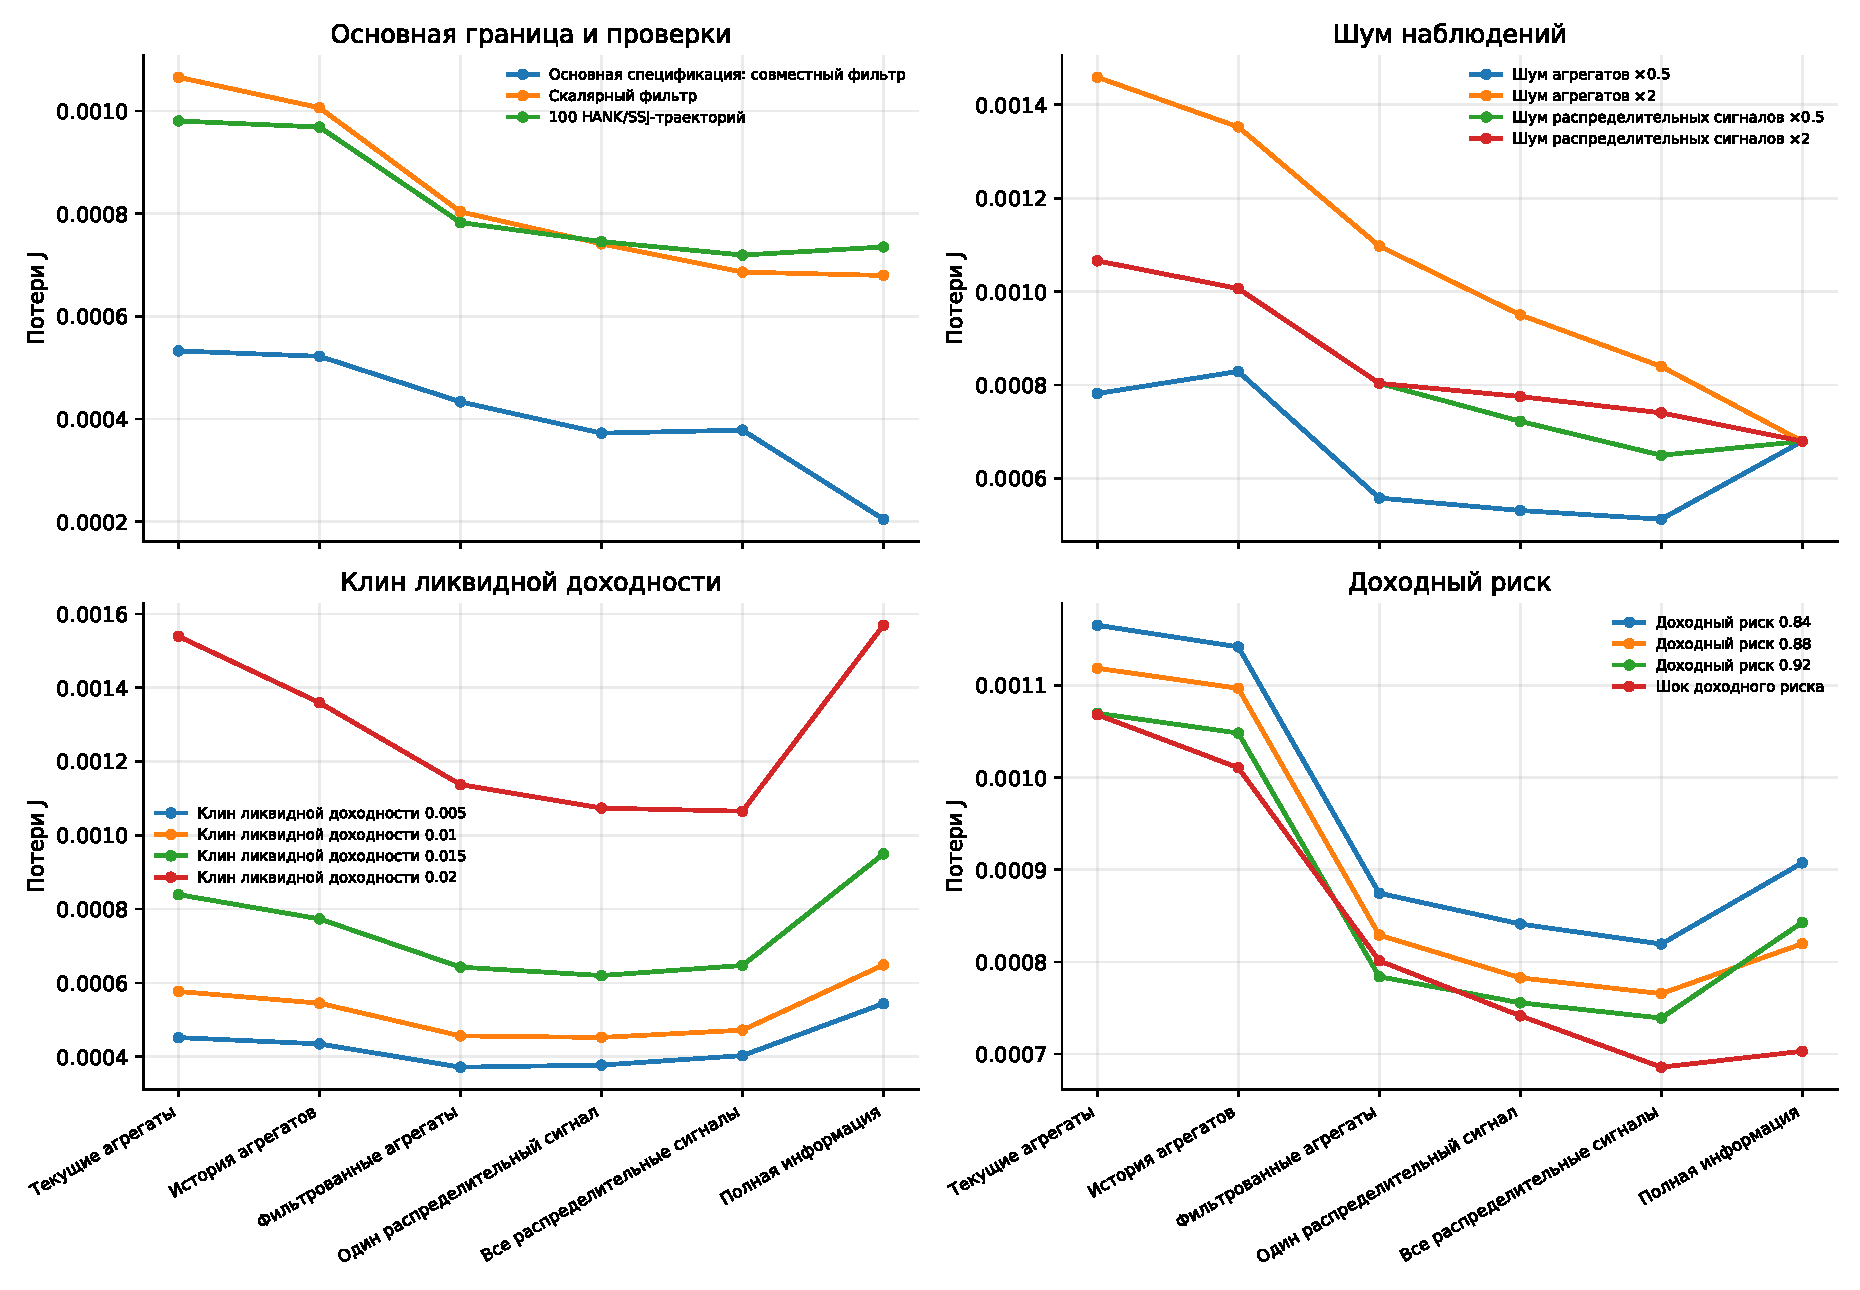
\includegraphics[width=\textwidth]{figures/fig_information_frontier.pdf}
\caption{Информационная граница: потери по уровням доступной информации}
\end{figure}

\begin{figure}[h!]
\centering
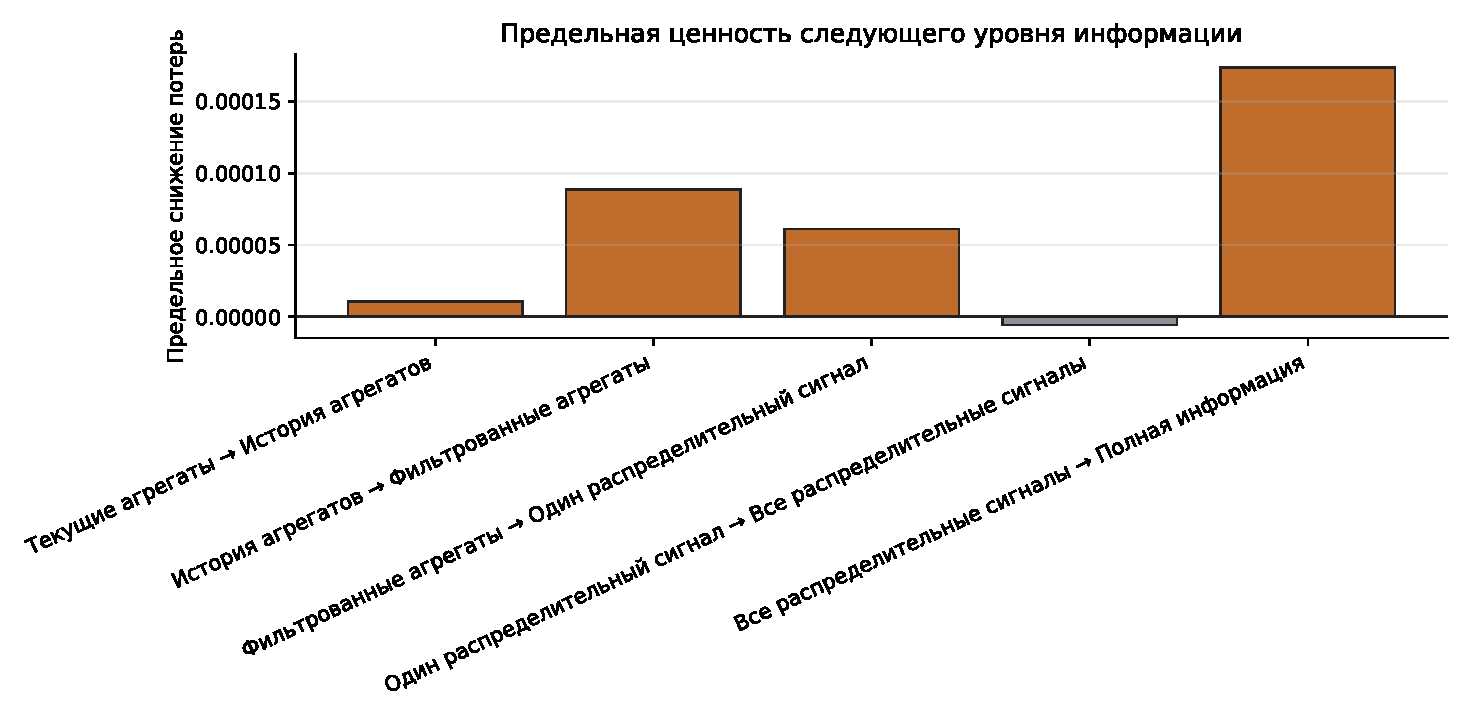
\includegraphics[width=\textwidth]{figures/fig_information_marginal_values.pdf}
\caption{Предельная ценность следующего уровня информации}
\end{figure}

\begin{table}[h!]
\centering
\caption{Устойчивость ранжирования информационных уровней}
\resizebox{\textwidth}{!}{%
\begin{tabular}{lrrrr}
\toprule
Проверка & Число вариантов & Средняя ранговая корреляция & Минимальная корреляция & Совпадение лучшего уровня \\
\midrule
Тестовые seed & 6 & 0.950 & 0.800 & 0.667 \\
Совместный фильтр против скалярного & 1 & 0.900 & 0.900 & 0.000 \\
Число траекторий & 1 & 1.000 & 1.000 & 1.000 \\
Шум наблюдений & 4 & 0.975 & 0.900 & 1.000 \\
Клин ликвидной доходности & 4 & 0.750 & 0.600 & 0.250 \\
Доходный риск & 4 & 1.000 & 1.000 & 1.000 \\
Сила распределительного сигнала & 4 & 1.000 & 1.000 & 1.000 \\
\bottomrule
\end{tabular}
}
\end{table}

Ранговая проверка проводится по реализуемым информационным состояниям 0--4; полная информация
остаётся ориентиром, но не включается в ранги старых sensitivity-прогонов. Ранжирование в целом
устойчиво к числу траекторий, шуму наблюдений, доходному риску и силе распределительного сигнала.
Наиболее чувствительная часть -- калибровка клина ликвидной доходности: при слабом клине
распределительная информация может не улучшать правило, а при более сильном канале её ценность
становится положительной.

\subsection{Оптимизация правил}

Смена способа настройки правил существенно влияет на уровни потерь. Например, для фильтрованных
агрегатов старый поиск по сетке даёт test loss \(0.000776\), а непрерывная оптимизация --
\(0.000433\). Для фильтрованного распределительного состояния соответствующие значения равны
\(0.000842\) и \(0.000378\). Поэтому в основной таблице используются результаты непрерывной
оптимизации, а таблица устойчивости сохраняет также старые режимы подбора.

Отдельная проверка показывает, что выигрыш распределительного состояния не является простой
проекцией коэффициентов. Если взять правило, настроенное на распределительном наборе, занулить
распределительные коэффициенты и применить его к фильтрованным агрегатам, средние потери равны
\(0.001858\), тогда как заново настроенное агрегатное правило даёт \(0.000433\). Это подтверждает,
что разные информационные состояния нужно сравнивать после отдельной настройки правила.

\subsection{Устойчивость к классу правила}

Основной результат не должен зависеть от одного специфического класса правил. Поэтому дополнительно
сравниваются несколько разумных альтернатив: правило типа Тейлора, правило Тейлора с потреблением,
правило Тейлора с распределительными показателями, правило с ограничениями на знаки, регуляризованные
линейные правила и малое нелинейное правило. Во всех случаях правила настраиваются на тех же
валидационных траекториях и оцениваются на тех же тестовых траекториях.

\begin{table}[h!]
\centering
\caption{Устойчивость ценности распределительной информации к классу правила}
\resizebox{\textwidth}{!}{%
\begin{tabular}{lrrrr}
\toprule
Класс правила & Снижение потерь & Нижняя граница для \(\Delta J\) & Верхняя граница для \(\Delta J\) & Доля выигрышей \\
\midrule
Правило Тейлора & 0.000058 & -0.000090 & -0.000025 & 0.560 \\
Тейлор + потребление & 0.000079 & -0.000103 & -0.000055 & 0.593 \\
Тейлор + распределительные показатели & 0.000141 & -0.000181 & -0.000103 & 0.610 \\
Правило с ограничениями на знаки & 0.000141 & -0.000181 & -0.000103 & 0.610 \\
Оптимизированное линейное правило & 0.000073 & -0.000101 & -0.000045 & 0.563 \\
Ridge-регуляризация & 0.000073 & -0.000101 & -0.000045 & 0.563 \\
LASSO/ElasticNet & 0.000073 & -0.000101 & -0.000045 & 0.563 \\
\bottomrule
\end{tabular}
}
\end{table}

Во всех основных классах правил предельная ценность распределительной информации остаётся
положительной. Это важно для интерпретации: результат не держится на одной форме линейного правила
и не исчезает при ограничениях на знаки или регуляризации коэффициентов. Малое нелинейное правило
используется только как дополнительная проверка; в текущей реализации оно даёт худший результат и
поэтому не является частью основного аргумента. Тем самым вывод работы остаётся не про преимущество
сложных алгоритмов, а про ценность информационного состояния.

\begin{figure}[h!]
\centering
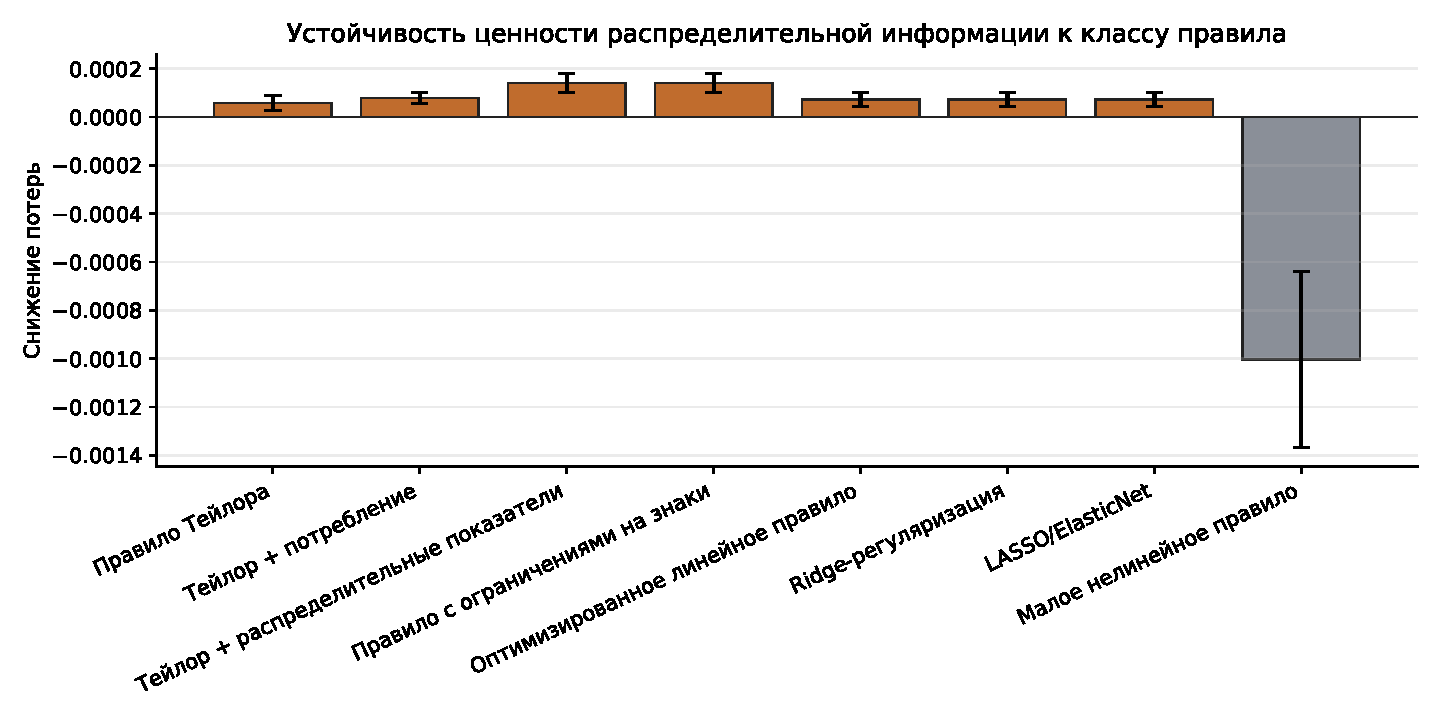
\includegraphics[width=\textwidth]{figures/fig_policy_class_robustness.pdf}
\caption{Снижение потерь при добавлении распределительной информации в разных классах правил}
\end{figure}

\subsection{Идентификационные проверки}

Чтобы отделить ценность информации от механического увеличения числа признаков, проводится
батарея проверок. Во всех вариантах агрегатный блок \(E\pi,EY,EC\) в распределительном
информационном состоянии принудительно приравнен к фильтрованным агрегатам. Меняются только
распределительные признаки.

\begin{table}[h!]
\centering
\caption{Идентификационные проверки распределительных признаков}
\resizebox{\textwidth}{!}{%
\begin{tabular}{lrrrr}
\toprule
Проверка & Снижение потерь & Нижняя граница для \(\Delta J\) & Верхняя граница для \(\Delta J\) & Доля выигрышей \\
\midrule
Фактическая распределительная информация & 0.000038 & -0.000070 & -0.000004 & 0.550 \\
Искусственные признаки с похожей статистикой & -0.000018 & 0.000008 & 0.000029 & 0.440 \\
Перемешивание между сценариями & 0.000003 & -0.000006 & -0.000000 & 0.540 \\
Перемешивание времени внутри сценария & 0.000002 & -0.000008 & 0.000005 & 0.590 \\
Запаздывающие распределительные признаки & -0.000027 & 0.000014 & 0.000040 & 0.393 \\
Будущие сдвинутые распределительные признаки & -0.000030 & 0.000018 & 0.000044 & 0.407 \\
Остаточная распределительная информация & 0.000055 & -0.000084 & -0.000025 & 0.563 \\
\bottomrule
\end{tabular}
}
\end{table}

Ключевой результат здесь -- строка с остаточной распределительной информацией. В ней
распределительные признаки предварительно очищаются от линейной зависимости от фильтрованных
агрегатов на валидационной выборке. Даже после этого снижение потерь остаётся положительным:
\(0.000055\), а интервал для \(\Delta J\) лежит ниже нуля. Напротив, искусственные признаки с
похожей дисперсией, авторегрессией и корреляцией с агрегатами ухудшают правило. Лаговые и
будущие сдвинутые признаки также ухудшают результат. Это говорит против объяснения «правило
выиграло просто потому, что получило больше входов».

\subsection{Сравнительная статика робастности}

Робастность удобно читать не как набор отдельных таблиц, а как ответы на три экономических
вопроса.

Первый вопрос: когда распределительная информация полезна? В старой sensitivity-спецификации при
росте шума агрегатных наблюдений предельная ценность распределительной информации возрастает:
при половинном шуме агрегатов \(MVOI_{dist}=0.000045\), а при удвоенном шуме агрегатов --
\(0.000258\). Напротив, когда шум самих распределительных сигналов растёт, ценность падает:
при половинном шуме распределительных сигналов \(MVOI_{dist}=0.000154\), при удвоенном --
\(0.000063\). Это соответствует основной гипотезе: распределительная информация ценна тогда,
когда она помогает компенсировать неполноту агрегатных сигналов, но сама должна быть достаточно
информативной.

Второй вопрос: когда распределительная информация не полезна? Если распределительная динамика
выключена, \(MVOI_{dist}\) исчезает. При слабом клине ликвидной доходности результат также
отрицателен или близок к нулю: при \(\omega=0.005\) \(MVOI_{dist}=-0.000031\), при
\(\omega=0.010\) -- \(-0.000016\), при \(\omega=0.015\) -- \(-0.000004\). При более сильном
канале, \(\omega=0.020\), показатель становится положительным и равен \(0.000072\). Поэтому
отрицательные случаи не являются провалом результата: они показывают, что распределительная
информация ценна не всегда, а именно когда распределительный канал достаточно силён.

Третий вопрос: через какой компонент функции потерь проходит выигрыш? В основной joint-filter
спецификации почти весь выигрыш от распределительной информации сверх фильтрованных агрегатов
идёт через разрыв выпуска. Из общего снижения \(0.000055\) около \(0.000048\) приходится на
компонент выпуска, тогда как инфляция даёт \(0.000004\), потребление -- \(0.000004\), а
сглаживание ставки почти не меняется. Экономически это означает, что распределительные сигналы
помогают не за счёт более агрессивной ставки, а за счёт лучшего выбора реакции на будущую
реальную трансмиссию.

\begin{figure}[h!]
\centering
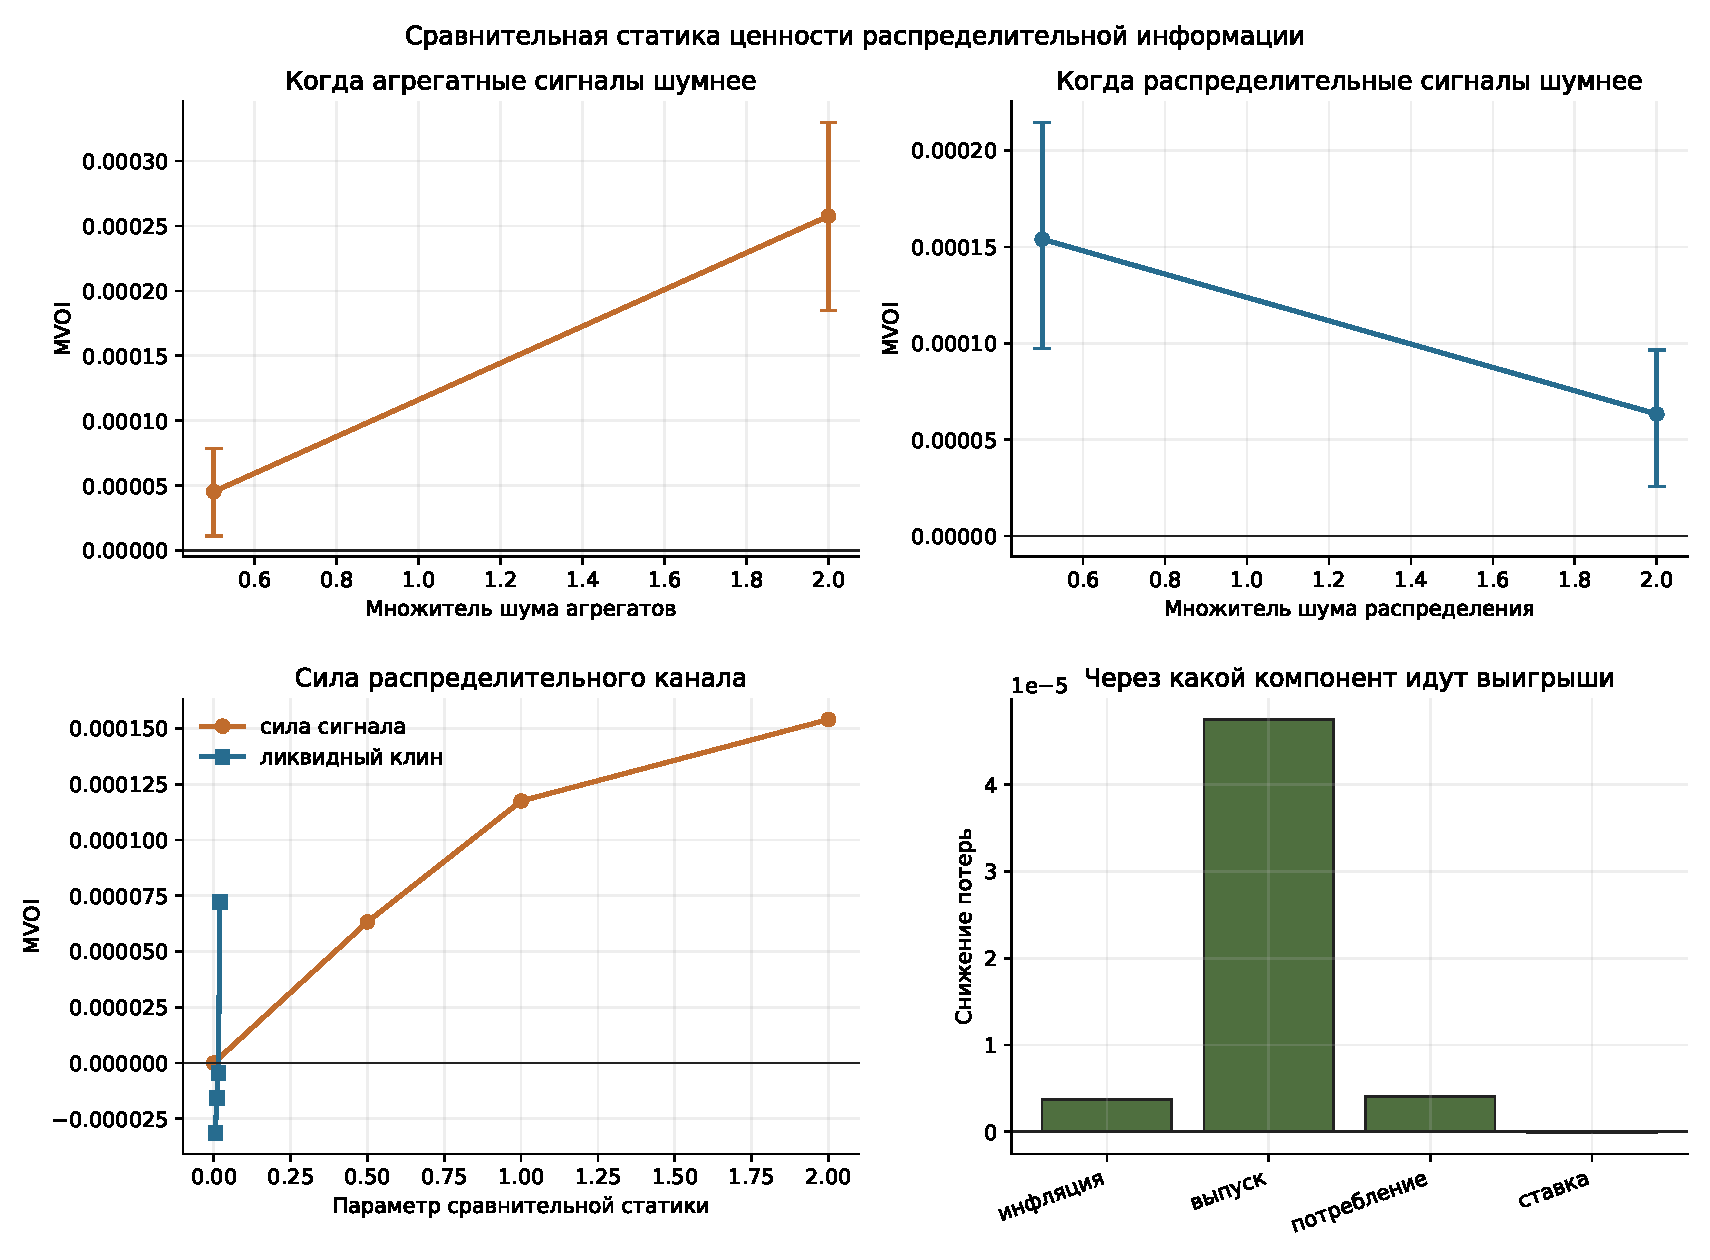
\includegraphics[width=\textwidth]{figures/fig_robustness_comparative_statics.pdf}
\caption{Сравнительная статика ценности распределительной информации}
\end{figure}

Часть сравнительной статики была посчитана в старой скалярной фильтровой спецификации. Поэтому
эти проверки используются как направленная экономическая робастность, а не как замена основной
оценки. Основная оценка статьи остаётся спецификацией с совместным фильтром Калмана и
непрерывной настройкой линейных правил.

\subsection{Механизм через локально оптимальную ставку}

Для проверки механизма строится локально SSJ-оптимальная траектория ставки \(i_t^{*,SSJ}\).
Затем оценивается, какие информационные состояния лучше предсказывают эту ставку на независимых
траекториях.

\begin{table}[h!]
\centering
\caption{Прогноз локально SSJ-оптимальной ставки}
\resizebox{\textwidth}{!}{%
\begin{tabular}{lrrrrr}
\toprule
Спецификация & RMSE & OOS \(R^2\) & \(\Delta\)RMSE vs aggregates & p-value & Directional accuracy \\
\midrule
Фильтрованные агрегаты & 0.000945 & 0.067 &  &  & 0.582 \\
Фильтрованные агрегаты + MPC & 0.000937 & 0.084 & -0.000008 & 0.00025 & 0.596 \\
Фильтрованные агрегаты + низкая ликвидность & 0.000936 & 0.085 & -0.000009 & 0.00025 & 0.599 \\
Фильтрованные агрегаты + процентная экспозиция & 0.000937 & 0.084 & -0.000009 & 0.00025 & 0.597 \\
Фильтрованные распределительные показатели & 0.000924 & 0.109 & -0.000022 & 0.00025 & 0.610 \\
\bottomrule
\end{tabular}
}
\end{table}

Распределительные признаки улучшают прогноз локально оптимальной ставки сверх фильтрованных
агрегатов. Полное распределительное состояние снижает RMSE с \(0.000945\) до \(0.000924\) и
повышает вневыборочный \(R^2\) с \(0.067\) до \(0.109\). После удаления части оптимальной ставки,
объясняемой агрегатами, остаточные распределительные признаки всё ещё объясняют около \(2.9\%\)
остаточной вариации.

\begin{figure}[h!]
\centering
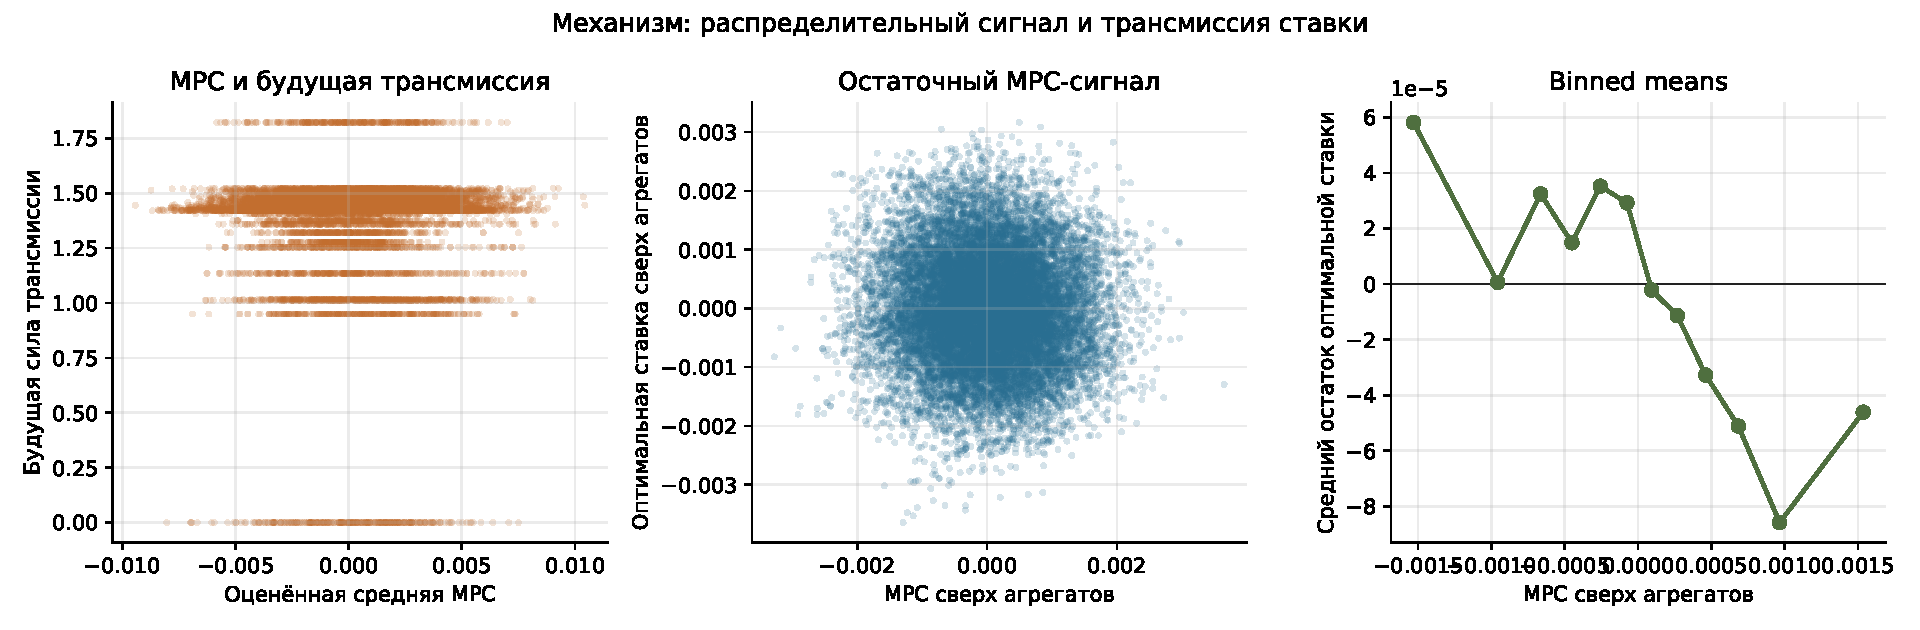
\includegraphics[width=\textwidth]{figures/fig_mechanism_distribution_transmission.pdf}
\caption{Распределительный сигнал, будущая трансмиссия и остаток оптимальной ставки}
\end{figure}

\begin{figure}[h!]
\centering
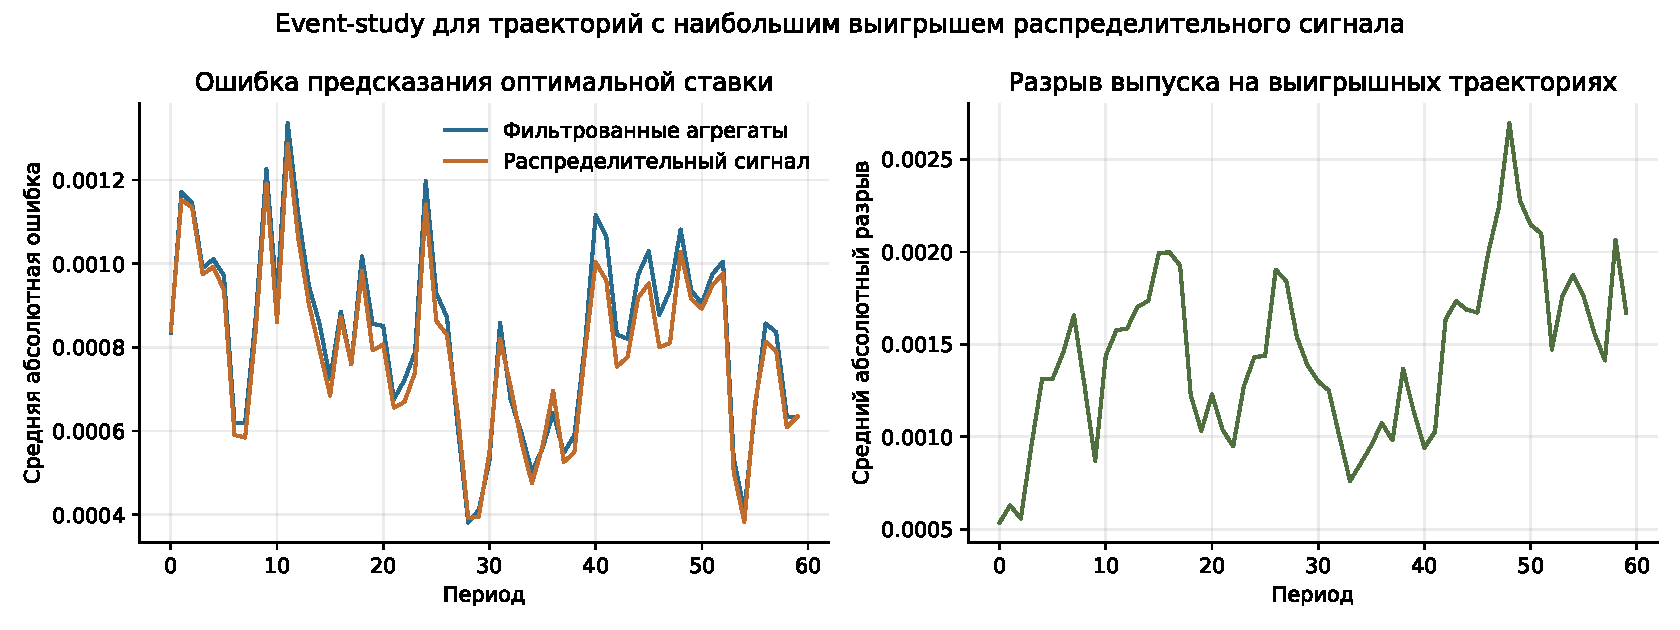
\includegraphics[width=\textwidth]{figures/fig_mechanism_event_study.pdf}
\caption{Траектории с наибольшим выигрышем распределительного сигнала}
\end{figure}

\subsection{Разложение потерь}

Разложение показывает, что основная часть выигрыша идёт через выпуск. При переходе от текущих
агрегатов к фильтрованным агрегатам общее снижение потерь равно \(0.000099\), из них
\(0.000074\) приходится на разрыв выпуска. При добавлении распределительной информации сверх
фильтрованных агрегатов общее снижение равно \(0.000055\), из них \(0.000048\) приходится на
разрыв выпуска. Компонент сглаживания ставки почти не меняется.

\subsection{Проверка с обратной связью}

В базовой локальной проекции информационные признаки берутся с исходной HANK/SSJ-траектории, а
агрегатные последствия альтернативной ставки пересчитываются через SSJ-отклики. В усиленной
проверке контрфактическое состояние, наблюдения и фильтрованные признаки пересчитываются
итеративно. Правила не переобучаются.

В режиме с обратной связью фильтрованные агрегаты дают средние потери \(0.002138\), а
фильтрованные распределительные показатели -- \(0.002098\). Знак остаётся правильным, но эффект
статистически слабее: снижение потерь равно \(0.000040\), а интервал для разности включает ноль.
Отдельные распределительные статистики выглядят устойчивее: доля низколиквидных домохозяйств и
процентная экспозиция снижают потери примерно на \(0.00031\) относительно фильтрованных агрегатов.

Эта проверка не является полной HANK-оценкой с обратной связью. В текущем наборе SSJ-якобианов
прямые отклики ставки есть для инфляции, выпуска и потребления, но не для распределительных
статистик. Поэтому для распределительных переменных используется локальная проекция на агрегатные
SSJ-эффекты. Максимальная следующая версия требует прямых SSJ-якобианов для MPC, доли
низколиквидных домохозяйств и процентной экспозиции.

\subsection{Интерпретация}

Абсолютные значения функции потерь малы, потому что эксперимент проводится вокруг стационарного
состояния и использует квадратичный стабилизационный критерий. Поэтому содержательная проверка
опирается на парные разности на одинаковых траекториях, доверительные интервалы, проверки с
ложными признаками и сравнение с полной информацией.

Итоговый вывод такой: распределительная информация имеет положительную предельную ценность в
локальной HANK/SSJ-среде, но эта ценность не должна трактоваться как автоматическое преимущество
любого расширенного набора переменных. Эффект сохраняется для остаточной распределительной
информации и исчезает или меняет знак для искусственных и временно смещённых признаков.

\section{Заключение}

Работа оценивает предельную информационную ценность распределительных статистик домохозяйств для
правила процентной ставки при неполной наблюдаемости в локальной HANK/SSJ-среде. В текущей версии
основной технической спецификацией является совместный фильтр Калмана: агрегатные и
распределительные оценки строятся из одной линейной модели состояния, а информационные режимы
различаются только матрицей наблюдения.

Отдельная конечная разностная проверка поддерживает локальную SSJ-аппроксимацию в используемом
диапазоне шоков. Экспортированный якобиан денежного шока даёт малую среднюю ошибку относительно
нелинейного HANK-перехода, а неполитические шоки также демонстрируют небольшие ошибки локальной
линейности. Это не превращает расчёт в глобальную нелинейную HANK-оценку, но делает локальную
интерпретацию результатов существенно более защищённой.

Главный устойчивый результат состоит в том, что восстановление агрегатного состояния существенно
снижает потери относительно текущих шумных агрегатов. Распределительная информация даёт
дополнительный, но умеренный выигрыш сверх фильтрованных агрегатов в базовой парной оценке и в
ряде идентификационных проверок. Однако large-sample проверка с отдельными HANK/SSJ-шоками и
кластеризацией по макрошоку делает этот вывод осторожнее: полный распределительный блок уже не
имеет статистически устойчивого выигрыша сверх фильтрованных агрегатов, тогда как отдельные
распределительные статистики сохраняют положительный, но слабый знак.

Идентификационные проверки показывают, что этот результат не сводится к механическому увеличению
числа признаков. Искусственные признаки с похожей дисперсией, авторегрессией и корреляцией с
агрегатами не воспроизводят выигрыш; временно сдвинутые признаки ухудшают правило. При этом
остаточная распределительная информация, очищенная от линейной зависимости от фильтрованных
агрегатов, сохраняет положительный эффект в базовом тесте. Более аккуратный вывод таков:
распределительные статистики могут быть самостоятельным источником информации для правила ставки,
если они помогают оценивать будущую трансмиссию ставки сверх уже восстановленного агрегатного
состояния, но этот канал в текущей калибровке не является настолько сильным, чтобы полный
распределительный блок устойчиво проходил large-sample кластерную проверку. Это именно локальный
результат HANK/SSJ-эксперимента, а не решение глобальной нелинейной задачи оптимальной политики в
полной HANK-модели.

Проверка с обратной связью усиливает этот вывод для локальной SSJ-постановки. После добавления
прямых HANK-откликов распределительных статистик на траекторию ставки полное распределительное
состояние устойчиво снижает потери относительно фильтрованных агрегатов. При этом результат
остаётся локальным: это не глобальная нелинейная HANK-оптимизация, а проверка замороженных правил в
локальной проекции вокруг стационарного состояния.

Поэтому финальная позиция работы не состоит в том, что распределительная информация всегда нужна
для денежно-кредитной политики. Более защищаемый вывод другой: в локальной HANK/SSJ-среде
агрегатная фильтрация является устойчиво ценной, а распределительные статистики имеют потенциальную
предельную ценность в тех спецификациях, где они несут информацию о будущей трансмиссии ставки.
Наиболее сильное подтверждение этого канала получается в closed-loop проверке с прямыми
распределительными SSJ-откликами; наиболее осторожный результат -- в large-sample проверке
открытой локальной проекции, где полный распределительный блок не проходит кластерную проверку.


\bibliographystyle{plain}
\bibliography{references}

\end{document}
